\documentclass[11pt]{article}
\usepackage[letterpaper, margin=1in]{geometry}

% Proper links
\usepackage[
    pdftitle={SYSC3010 Computer Systems Development Project - FANS Project Proposal},
    colorlinks=false,
    allbordercolors={0 0 0},
    citebordercolor={1 1 1}, % No border for citations
    pdfborderstyle={/S/U/W 1},
]{hyperref}

% Display graphics nicely
\usepackage{float}
\usepackage{graphicx}

% References
\usepackage[style=ieee]{biblatex}
\addbibresource{./references.bib}

% Remove paragraph indentation and use newline to separate instead. %
\usepackage[parfill]{parskip}
\setlength{\parindent}{0cm}

\author{
    Grant Achuzia, 101222695 \\
    Javeria Sohail, 101197163 \\
    Matteo Golin, 101220709 \\
    Saja Fawagreh, 101217326 \\
    TA: Sean Kirkby
}
\title{
    SYSC3010 Computer Systems Development Project \\
    FANS Detailed Design Report \\
    {\large Group L1-G8} \\
    {
        \vspace{0.5in}
        \centering
        
\includegraphics[width=4in]{../assets/header-image.jpg} \\
        \small \cite{header-img}
    }
}
\date{
    Created: March 11th, 2024 \\
    Modified: \today
}

\begin{document}

% TITLE %
\maketitle
\pagebreak

% TABLE OF CONTENTS %
{
    \hypersetup{hidelinks}
    \tableofcontents
}

% MAIN MATTER %
\section{Project Description}

\subsection{Motivation}

The motivation for the FANS project was to address the critical problem of preventable fire-related deaths in Canada.
Fire safety was a fundamental concern for individuals, families, and communities nationwide. By leveraging modern
technological advancements, the FANS system aimed to significantly enhance the effectiveness of fire alarm systems,
reducing response times, and ultimately saving lives. The importance of this project could not be overstated, as it
directly impacted the safety and well-being of Canadians.

\subsection{Problem Statement}

The need for the Fire Alarm Notification System (FANS) stemmed from the alarming number of preventable fire deaths in
Canada, where 220 people died in fires each year, with at least one in seven of these deaths occurring in homes without
working smoke alarms \cite{fire-stats}. This critical problem underscored the shortcomings of traditional fire alarm
systems, which often lacked advanced communication capabilities and real-time monitoring capabilities
\cite{modern-fire-alarms}. These limitations not only contributed to delayed response times but also to preventable
deaths, underscoring the urgent need for an advanced fire alarm solution.

Traditional systems’ shortcomings, coupled with the fact that smoke detection systems were sometimes unsafely disarmed
by users to avoid false alarms—especially those installed close to kitchen spaces—further exacerbated the problem. The
FANS project sought to address these issues by integrating smoke and temperature sensors with Internet of Things (IoT)
technology. This approach not only aimed to cover scenarios where smoke may not reach the detecting device but also
offered real-time notifications via SMS and email, thus notifying homeowners immediately in the event of an emergency.

By providing configurable thresholds for smoke and temperature alarms and adjustable timeouts that prevented the system
from being deactivated in an unsafe manner, FANS aimed to use technological advances to significantly improve the
effectiveness of fire detection systems. The ultimate goal of the project was to reduce response times, improve overall
fire safety, and thereby mitigate fire disasters and protect the well-being of individuals, families, and communities
across Canada \cite{smoke-alarm-gc}.

\subsection{Overview of Solution}

\section{Design Overview}

The Fire Alarm Notification System (FANS) is a real-time system designed for efficient fire detection and alerting. The
system is composed of several key components, each with a distinct function but integrated to work seamlessly together,
ensuring a comprehensive approach to fire safety. The system's architecture is outlined in a detailed deployment
diagram in Figure \ref{fig:deployment}, illustrating the interconnections between the various components. These
components include:

\begin{itemize}
    \item \textbf{Alarm System:} Based on a Raspberry Pi 4, this system triggers audible and visual alerts in the event
          of a fire, ensuring that occupants are promptly warned.

    \item \textbf{Smoke Detection System:} Also utilizing a Raspberry Pi 4, this system constantly monitors the
          environment for smoke using advanced sensors. It is the primary detection mechanism that activates the alarm
          system and notification system upon detecting smoke.

    \item \textbf{Notification System:} Operating on a Raspberry Pi 4, this system sends out emergency alerts to
          predefined contacts, including both local authorities and individuals, ensuring rapid response to the detected
          fire.

    \item \textbf{Cloud Database:} A real-time cloud database is employed to store critical data, including sensor
          readings (smoke and temperature levels) and system configurations. This facilitates remote monitoring and
          configuration, ensuring that the system is always functioning optimally.

    \item \textbf{Haptic Alarm:} This device provides haptic feedback, offering an additional layer of alert through
          physical sensation, ensuring that even those who may not be within hearing range of the alarm or have hearing
          impairments are alerted.

    \item \textbf{User Interface:} A web-based application for monitoring the system's environment and configuring
          system settings.
\end{itemize}

The system's design emphasizes scalability, allowing for easy expansion with additional sensors or alarm units as
needed. It also highlights modularity, where each component can function independently, ensuring reliability and ease
of maintenance. Communication between the components is facilitated through a local network, with the cloud database
supporting remote access and control.

Furthermore, the system incorporates advanced communication protocols for efficient data exchange and alerting. The
smoke detection system employs the I2C protocol for sensor communication, while UDP packets facilitate local network
communication between the system's nodes. HTTP requests are utilized for interactions with the cloud-hosted real-time
Firebase database, ensuring timely updates and access to system data.

Overall, the Fire Alarm Notification System is designed to be a reliable, efficient, and scalable solution for fire
detection and notification, leveraging modern technology to provide real-time alerts and ensuring the safety of
occupants in any building.

\subsection{System Overview Design}

\begin{figure}[H]
    \centering
    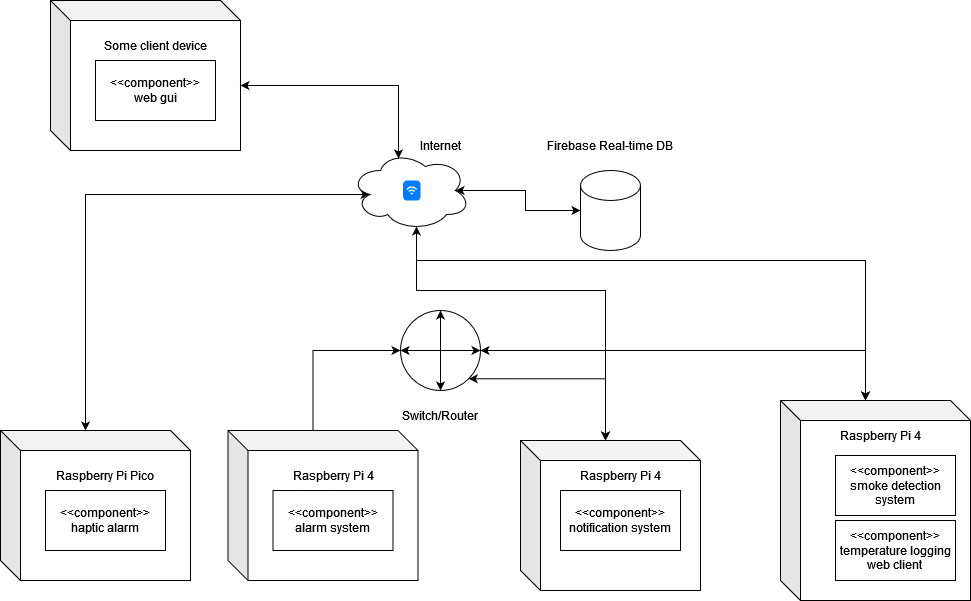
\includegraphics[width=\linewidth]{../assets/FANSDeployment.png}
    \caption{The deployment diagram for FANS.}
    \label{fig:deployment}
\end{figure}

\subsection{Communication Protocols}

In the Fire Alarm Notification System (FANS), a variety of communication protocols are meticulously integrated to
ensure seamless interaction among the system components and with the external cloud database, facilitating a robust and
responsive fire alarm solution.

The system's core, the Smoke Detection System, communicates with its temperature and smoke sensors using the I2C
protocol over the GPIO pins of a Raspberry Pi 4. This protocol choice is pivotal for real-time data acquisition,
allowing the system to monitor environmental conditions continuously and detect any signs of fire immediately. For
interactions within the local network, including communication between the smoke detection system, the alarm system,
and the notification system, UDP packets are employed. This approach is selected for its efficiency and speed, ensuring
that critical data is transmitted quickly and reliably across the system components without the overhead of
establishing and maintaining a connection, which is crucial in emergency situations where every second counts.

The integration with the cloud is achieved through HTTP requests to a Firebase real-time database. This cloud database
is essential for storing sensor data, system configurations, and user information. It supports various operations,
including the posting of sensor data by the smoke detection system, retrieval of data for the web GUI, fetching contact
information for the notification system, and polling for emergency flags by the haptic alarm system. These interactions
are facilitated by HTTP's flexibility and its widespread support across internet infrastructure, enabling the FANS to
leverage cloud computing benefits for enhanced data management and accessibility.

Lastly, the notification system's ability to reach users through email and SMS text notifications is realized through
standard internet SMS and email protocols. This ensures that in the event of a fire, users are promptly informed
regardless of their location, providing critical information and instructions to enhance their safety and response
effectiveness.

Together, these communication protocols form the backbone of the Fire Alarm Notification System, enabling it to
function as a cohesive, efficient, and highly responsive fire safety solution.

The Fire Alarm Notification System (FANS) employs a variety of communication protocols to ensure seamless interactions
between its components and with the external cloud database. This section provides detailed tables describing each
communication pathway.

\subsubsection{I2C Communication}

The Raspberry Pi 4 utilizes the I2C protocol to communicate with an array of temperature and smoke sensors, monitoring
environmental conditions to detect potential fire hazards. This is not visible in the sequence diagrams as they show
the bigger picture of the communication of the nodes with the sensors.

\begin{table}[H]
    \centering
    \begin{tabular}{| c | c | c | c | c |}
        \hline
        Sender         & Receiver               & Message              & Data Format                                          & Protocol                 \\
        \hline
        Raspberry Pi 4 & Temperature Sensor     & \texttt{read\_temp}  & See section 6.2.1 of datasheet \cite{temp-datasheet} & I2C                      \\
        \hline
        Raspberry Pi 4 & Smoke Sensor (via ADC) & \texttt{read\_smoke} & See figure 1.1 of datasheet \cite{adc-datasheet}     & SPI \cite{adc-datasheet} \\
        \hline
    \end{tabular}
    \caption{Messages for I2C communication in FANS.}
\end{table}

\subsubsection{Local Area Network Communication}

Nodes within the FANS (smoke detection, alarm, and notification systems) communicate over a local network using UDP
packets, facilitating real-time alerts and system coordination.

The messages sent over UDP use numerical value to encode messages. The representation agreed upon is as follows:

\begin{table}[H]
    \centering
    \begin{tabular}{| c | c |}
        \hline
        Message      & Value \\
        \hline
        Emergency    & 0     \\
        \hline
        No Emergency & 1     \\
        \hline
    \end{tabular}
    \caption{Numerical representation of messages over UDP in FANS.}
\end{table}

\begin{table}[H]
    \centering
    \begin{tabular}{| c | c | c | c | c |}
        \hline
        Sender                 & Receiver            & Message      & Data Format & Protocol \\
        \hline
        Smoke detection system & Notification system & Emergency    & 0           & UDP      \\
        \hline
        Smoke detection system & Alarm system        & Emergency    & 0           & UDP      \\
        \hline
        Smoke detection system & Notification system & No emergency & 1           & UDP      \\
        \hline
        Smoke detection system & Alarm system        & No Emergency & 1           & UDP      \\
        \hline
    \end{tabular}
    \caption{Messages for local area network communication in FANS.}
\end{table}

\subsubsection{Cloud Database Communication}

\begin{table}[H]
    \centering
    \begin{tabular}{| c | c | c | c | c |}
        \hline
        Sender          & Receiver & Message                                    & Data Format                      & Protocol    \\
        \hline
        Smoke Detection & Cloud DB & \texttt{put\_sensor\_data()}               & See listing \ref{lst:sensor}     & HTTP (JSON) \\
        \hline
        GUI             & Cloud DB & \texttt{update\_threshold(new\_threshold)} & See listing \ref{lst:threshold}  & HTTP (JSON) \\
        \hline
        Notification    & Cloud DB & \texttt{query\_contact\_information()}     & See listing \ref{lst:contact}    & HTTP (JSON) \\
        \hline
        Haptic Alarm    & Cloud DB & \texttt{emergency()}                       & See listing \ref{lst:emergency}  & HTTP (JSON) \\
        \hline
        GUI             & Cloud DB & \texttt{get\_sensor\_data()}               & See listing \ref{lst:sensor-get} & HTTP (JSON) \\
        \hline
    \end{tabular}
    \caption{Messages for cloud database communication in FANS.}
\end{table}

\begin{lstlisting}[language=json,label={lst:sensor},caption={Update sensor data message.}]
{
  "method": "PUT",
  "path": "/sensor-data/temperature",
  "headers": {
    "Authorization": "Bearer YOUR_ACCESS_TOKEN",
    "Content-Type": "application/json"
  },
  "body": {
      "data": {
          "temperature": 21.2,
          "timestamp": "2024-03-13T08:37:22"
      }
  }
}
\end{lstlisting}

\begin{lstlisting}[language=json,label={lst:threshold},caption={Threshold update message.}]
{
  "method": "PUT",
  "path": "/system/threshold",
  "headers": {
    "Authorization": "Bearer YOUR_ACCESS_TOKEN",
    "Content-Type": "application/json"
  },
  "body": {
    "newThreshold": 50
  }
}
\end{lstlisting}

\begin{lstlisting}[language=json,label={lst:contact},caption={Request for user contact information.}]
{
  "method": "GET",
  "path": "/user/contact",
  "headers": {
    "Authorization": "Bearer YOUR_ACCESS_TOKEN"
  }
}
\end{lstlisting}

\begin{lstlisting}[language=json,label={lst:emergency},caption={Request for emergency flag.}]
{
  "method": "GET",
  "path": "/system/emergency",
  "headers": {
    "Authorization": "Bearer YOUR_ACCESS_TOKEN"
  }
}
\end{lstlisting}

\begin{lstlisting}[language=json,label={lst:sensor-get},caption={Request for latest sensor data.}]
{
  "method": "GET",
  "path": "/sensor-data",
  "headers": {
    "Authorization": "Bearer YOUR_ACCESS_TOKEN"
  }
}
\end{lstlisting}

\subsubsection{User Notification Communication}

The notification system communicates with users through email, employing standard internet protocols to ensure timely
and effective alerts.

\begin{table}[H]
    \centering
    \begin{tabular}{| c | c | c | c | c |}
        \hline
        Sender              & Receiver   & Message                & Data Format                 & Protocol     \\
        \hline
        Notification System & User Inbox & Emergency notification & See listing \ref{lst:email} & SMTP (Email) \\
        \hline
    \end{tabular}
    \caption{Messages for user notification communication in FANS.}
\end{table}

\begin{lstlisting}[label={lst:email},caption={Email notification for detected emergency in FANS.}]
FROM: notification@example.com
TO: user@example.com
SUBJECT: Fire Alarm Notification

Dear [User's Name],

Fire alarm detected. Evacuate immediately.

- Location: [Location]
- Date/Time: [Date/Time]

Stay safe!
\end{lstlisting}

\subsection{Message Sequence Diagrams}

To implement the functional requirements described in Section 1.1: Functional Requirements, the FANS system will
satisfy six core use cases highlighted and illustrated in the message sequence diagrams below.

\subsubsection{Trigger Emergency Use Case}

The Trigger Emergency Use Case represents the critical functionality of the FANS, where the system detects a potential
fire through its smoke detection system and initiates a series of automated responses to mitigate the situation. As
depicted in the message sequence diagram, the process begins when the smoke detection system identifies smoke and
potentially high temperatures indicative of a fire. This detection triggers the system to send a notification to the
alarm system and the notification system. The alarm system responds by sounding an audible and visible alert to notify
occupants of the building immediately. Concurrently, the notification system sends out emergency alerts via SMS and
email to all registered users, ensuring they are informed of the danger regardless of their current location. This
response ensures that all the users are promptly alerted to the emergency, resulting in a quick evacuation and response
to the detected threat.

\begin{figure}[H]
    \centering
    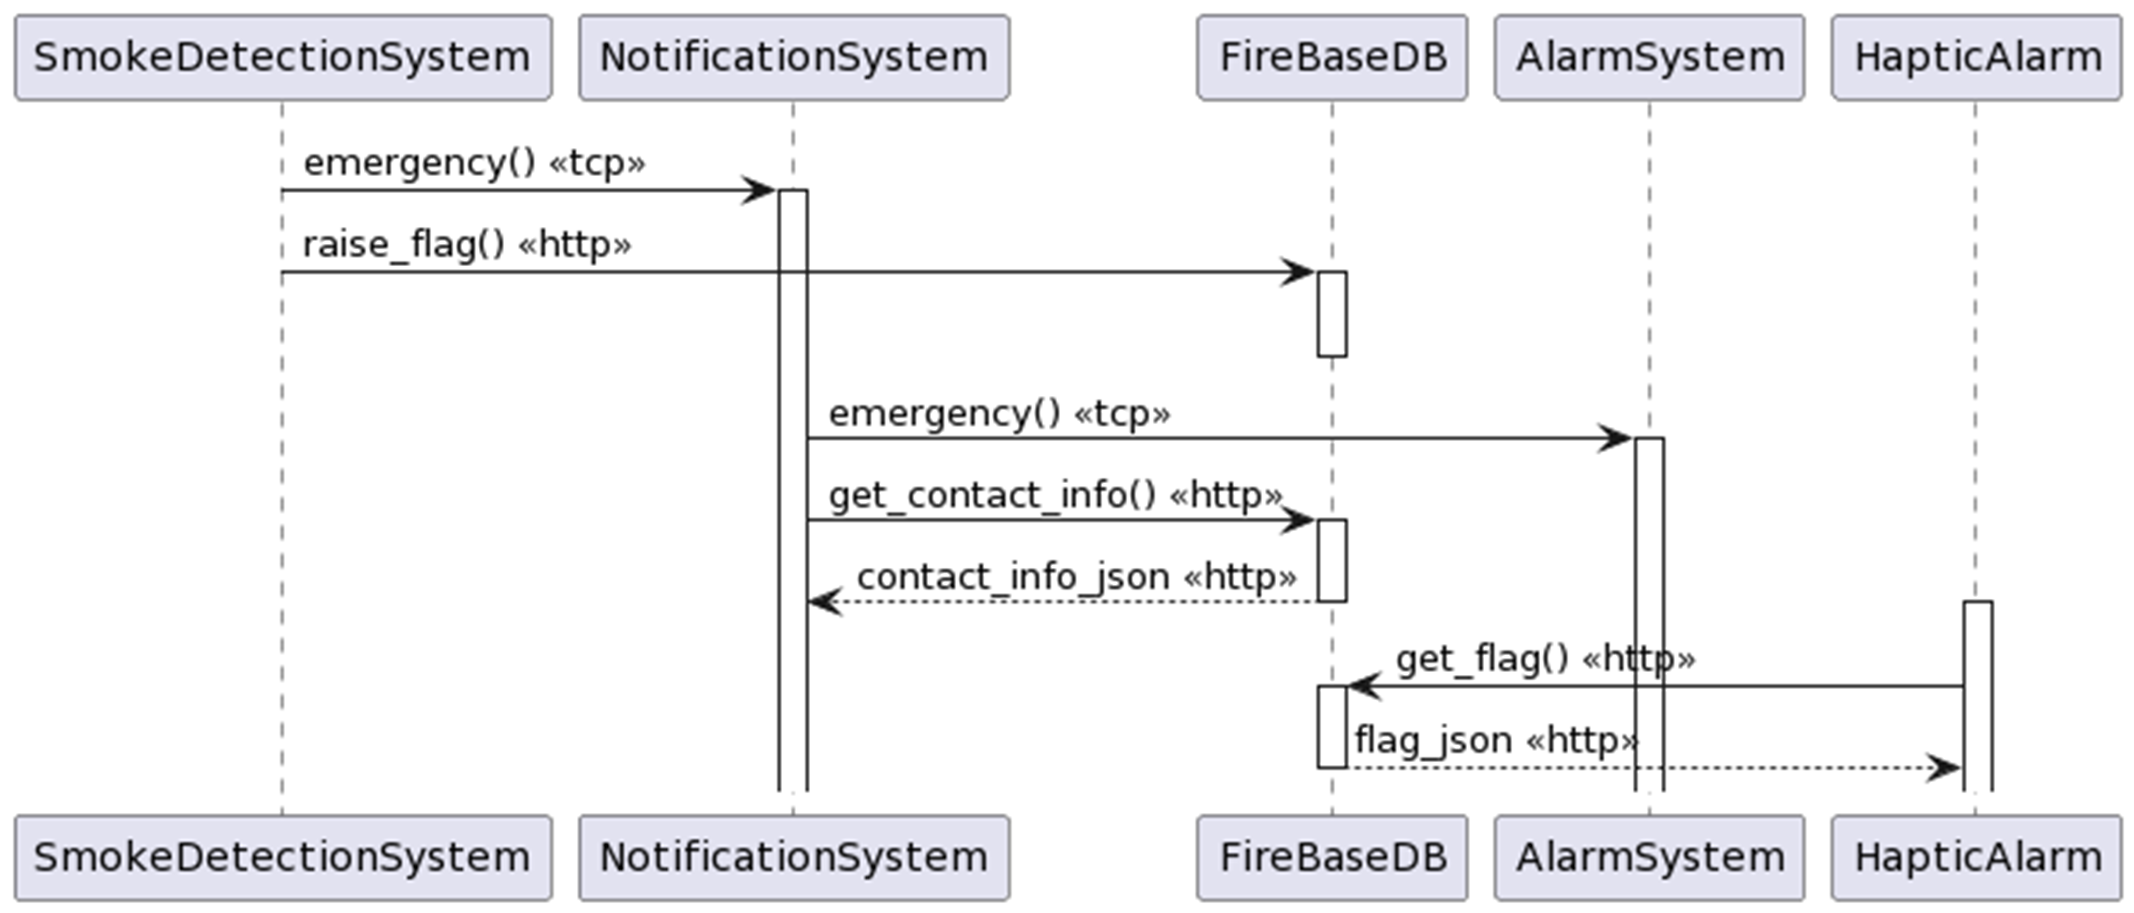
\includegraphics[width=\linewidth]{../assets/sequence/TriggerEmergencyUseCaseSequenceDiagram.png}
    \caption{Sequence diagram for the trigger emergency use case.}
\end{figure}

\subsubsection{Add New Contact Information Use Case}

This use case outlines the process by which users can add new contact information to the FANS database. Through the web
GUI, a user enters new contact details, such as phone numbers and email addresses, that the system can use to send
emergency notifications. Upon submission, these details are updated in the real-time database. The message sequence
diagram for this use case (not shown) illustrates the interactions between the user, the web GUI, and the database,
culminating in the notification system being updated with the new contact information. This ensures that the FANS can
reach the user through various channels in the event of an emergency, enhancing the system's effectiveness in
communicating critical alerts.

\begin{figure}[H]
    \centering
    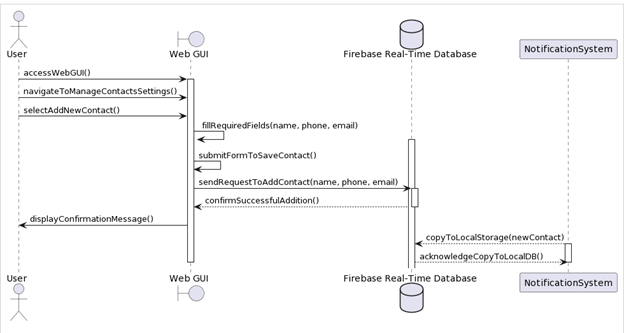
\includegraphics[width=\linewidth]{../assets/sequence/AddingNewContactInformationSequenceDiagram.png}
    \caption{Sequence diagram for the add contact info use case.}
\end{figure}

\subsubsection{Change Emergency Threshold Use Case}

Adjusting the smoke detection threshold is an essential feature that allows users to customize the sensitivity of the
FANS based on environmental conditions and personal preferences. This use case involves a user accessing the web GUI to
modify the threshold settings that determine when the smoke detection system should trigger an alert. The message
sequence diagram (not shown) visualizes the steps involved, from the user's interaction with the GUI to update the
threshold to the real-time database's role in storing this new setting. The smoke detection system then retrieves and
applies the updated threshold, ensuring that the FANS operates according to the user's specifications, balancing
sensitivity and false alarm minimization.

\begin{figure}[H]
    \centering
    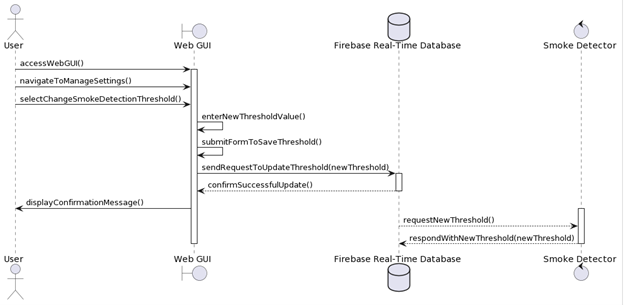
\includegraphics[width=\linewidth]{../assets/sequence/ChangingSmokeDetectionThresholdSequenceDiagram.png}
    \caption{Sequence diagram for the change threshold use case.}
\end{figure}

\subsubsection{Emergency Response Use Case}

This scenario highlights the FANS's capability to notify users in the event of a detected fire. Upon detecting a fire,
the notification system queries the cloud database for contact information and then sends out alerts via SMS and email
to all users. The message sequence diagram for this use case (provided above) captures the sequence of these
interactions, showcasing how the system ensures that occupants are informed and ready to address the emergency
promptly.

\begin{figure}[H]
    \centering
    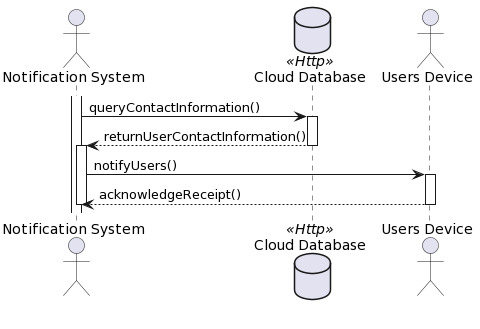
\includegraphics[width=\linewidth]{../assets/sequence/UserNotificationSequenceDiagram.png}
    \caption{Sequence diagram for the emergency response use case.}
\end{figure}

\subsection{Database Table Schema}

The FANS project will employ a Firebase Real-Time Database to store and manage data crucial for its operation. Given
the real-time nature of the FANS system, the choice of Firebase facilitates immediate updates and retrieval of data,
which is vital for emergency detection and notification. The data structure is designed to ensure efficient data
storage, retrieval, and management while supporting the scalability and real-time data processing requirements of the
system.

\begin{figure}[H]
    \centering
    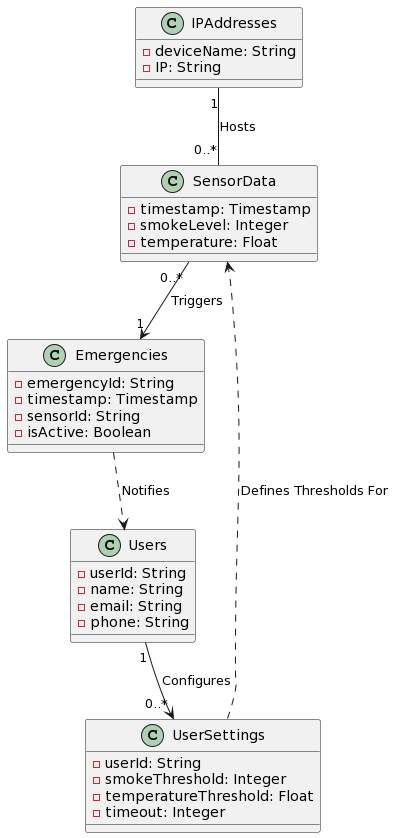
\includegraphics[width=3in]{../assets/class/DatabaseTableDesign.png}
    \caption{A visual of the FANS database design schema.}
\end{figure}

This schema optimizes the FANS system's performance by enabling efficient data storage, quick access to historical
data, and seamless integration between the system's components. The design also supports scalability, allowing for easy
addition of new sensors and users without significant alterations to the underlying database structure.

\section{Software Design}

Each node in the FANS system has its software design outlined below. Simple system nodes with an algorithmic design
have their control flow described using state machine diagrams as an aid. Class diagrams are included for nodes that
use an object-oriented approach for their design.

\subsection{Sensor Data Collection System}

The sensor collection system will be programmed using the Python programming language for simplicity and its large
collection of libraries.

The structure of the program will be that of two continuous polling loops, running as separate processes to utilize the
CPU fully and get around the Global Interpreter Lock (GIL) of Python that prevents maximizing traditional thread
performance.

The first polling loop will be responsible for collecting sensor data continuously and placing it on a queue for the
other loop. It will collect data from all sensors, and that is its sole responsibility.

\begin{figure}[H]
    \centering
    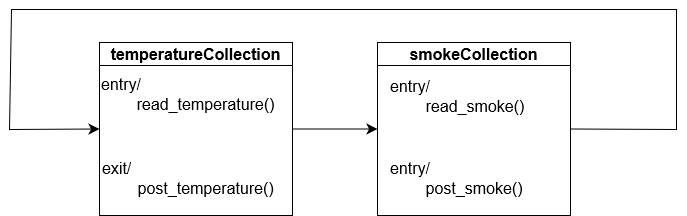
\includegraphics[width=\linewidth]{../assets/state-machine/DataCollectionStateMachine.png}
    \caption{The polling loop for sensor data collection.}
\end{figure}

The second polling loop will be responsible for reading the sensor data from the shared queue and writing it to the
Firebase database. It will also be responsible for performing logical checks on this data to determine whether or not
there is an active fire emergency. It will update the emergency flag in the database whenever a sensor data measurement
is above the specified threshold, and also communicate the emergency over UDP to the notification system and alarm
system. Once all sensor data has been posted to the database, this loop will check for configuration updates in the
sensor data thresholds from the Firebase database and apply them to the next iteration.

\begin{figure}[H]
    \centering
    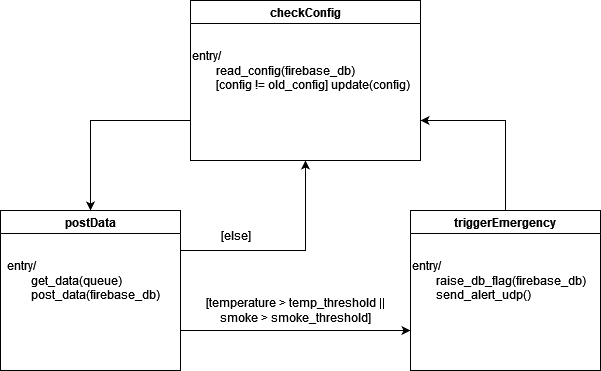
\includegraphics[width=\linewidth]{../assets/state-machine/DataCollectionLogicLoop.png}
    \caption{State machine diagram for the second process of the sensor data collection system.}
\end{figure}

\subsection{Alarm System}

The alarm system will be programmed using the Python programming language, again for its simplicity. The alarm system
will be composed of one continuous loop, which waits to receive incoming UDP messages. When a UDP message signifying an
emergency is received, the alarm system will trigger both an alarm buzzer and flashing LED lights for an infinite
duration. The alarm response will be interrupted only when the system receives another UDP message signifying that the
emergency has ended. This behaviour is similar to a state machine, so the software will be created using the state
design pattern.

\begin{figure}[H]
    \centering
    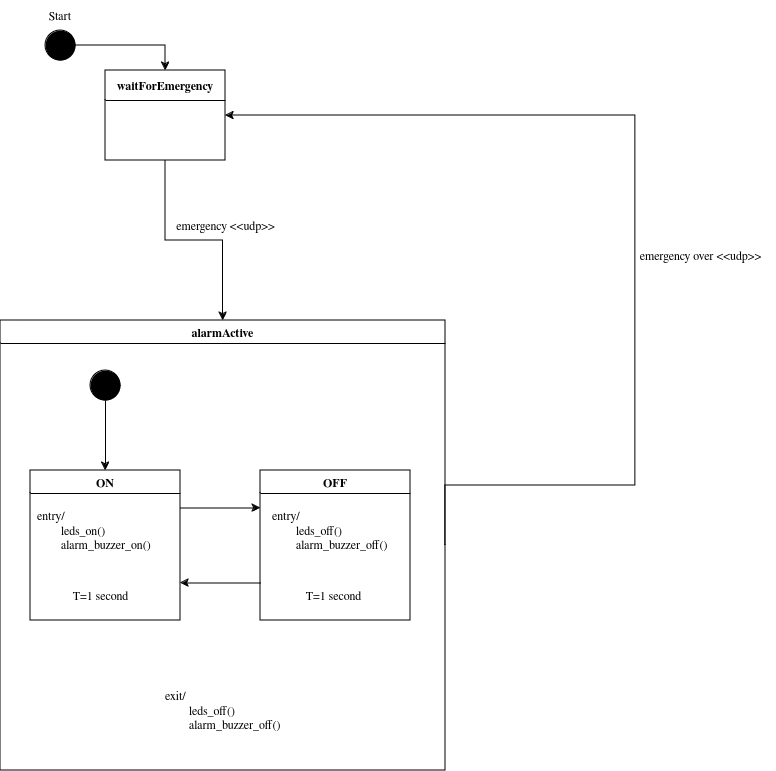
\includegraphics[width=\linewidth]{../assets/state-machine/AlarmSystemStateMachine.png}
    \caption{State machine diagram for the alarm system node.}
\end{figure}

\subsection{Notification System}

The notification system will be written in the Python programming language, also due to its simplicity and availability
of libraries for sending email notifications \cite{python-email}. The notification system will listen for a UDP message
signifying an emergency, and then send out email and SMS notifications to all users in the Firebase database. Once a
UDP message signifying the end of the emergency is received, the system will send a followup email to all users that
the emergency has been resolved.

\begin{figure}[H]
    \centering
    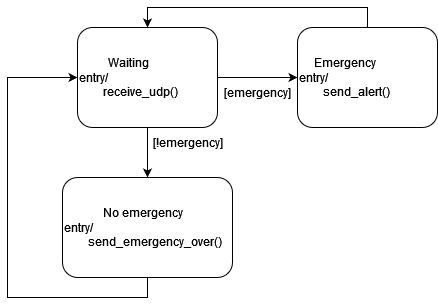
\includegraphics[width=4in]{../assets/state-machine/NotificationSystemStateMachine.png}
    \caption{The state machine representing the primary functionality of the notification system.}
\end{figure}

The notification system will keep a local cache of user contact information as a backup for failing internet
connectivity. It will periodically update its local cache with any changes in the upstream Firebase database.

The notification system will also have locally stored email and SMS templates for notifications. These will be loaded
as "Templates", which provide an interface for easy customization and sending of notifications.

\begin{figure}[H]
    \centering
    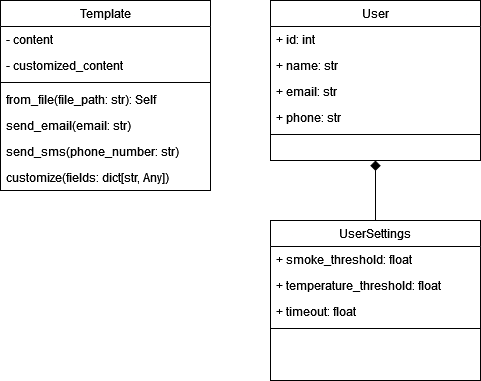
\includegraphics[width=3in]{../assets/class/NotificationSystemClassDiagram.png}
    \caption{Class diagram for the notification system node.}
\end{figure}

\subsection{Haptic Alarm System}

The haptic alarm wearable also has a very simple software design, and will be written in the Python programming
language. The program will continuously poll the Firebase database for changes in the emergency flag. Once the
emergency flag has been raised, the haptic alarm will begin to buzz on and off. During this time, it will continue
checking for changes in the emergency flag on the Firebase database. Once the emergency flag is lowered, the haptic
alarm will stop buzzing, signifying the end of the emergency.

\begin{figure}[H]
    \centering
    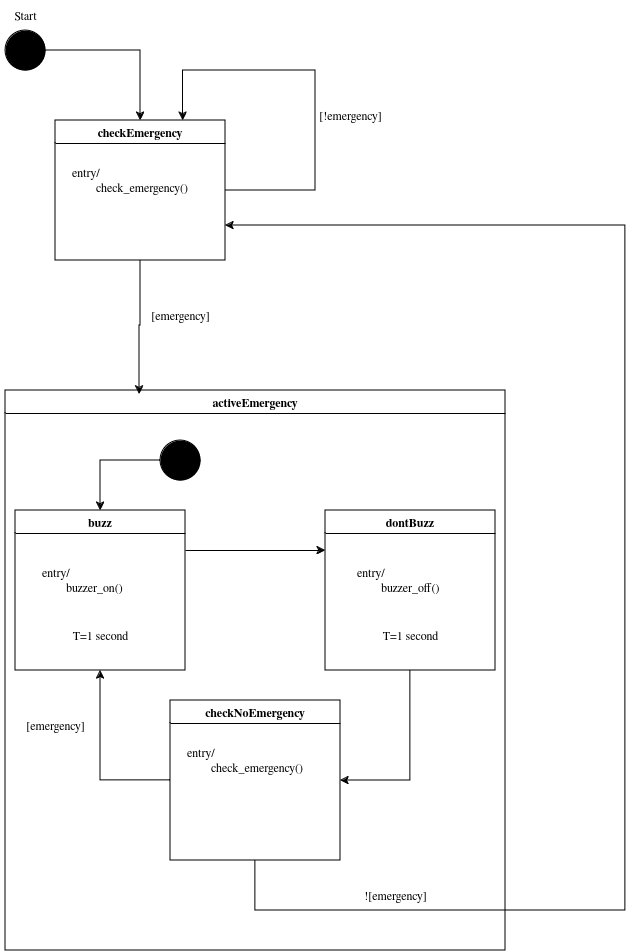
\includegraphics[width=4in]{../assets/state-machine/HapticAlarmStateMachine.png}
    \caption{State machine diagram for the haptic alarm system node.}
\end{figure}

\section{Hardware Design}

FANS is composed of various hardware components to perform its desired functionality.

\subsection{Raspberry Pi SenseHat}

The Raspberry Pi SenseHat is responsible for providing the temperature data readings collected by the smoke detection
system. This component was chosen because it's readily available and also has a large number of tutorials available for
integrating it into systems \cite{sensehat}. A diagram is not shown as the SenseHat is self-contained and can simply be
directly place on top of the Raspberry Pi 4, connected via the GPIO pin headers.

\subsection{MQ2 Smoke Sensor}

The MQ2 Smoke Sensor is a critical component in the FANS project, chosen for its capability to detect a wide range of
gases that occur, including smoke, which is essential for early fire detection. It operates at 5V and outputs an analog
signal that varies with the concentration of detected gases. The sensor's sensitivity to smoke enables the system to
promptly identify fire hazards, triggering alerts and activating safety measures. Its analog output necessitates an
analog-to-digital converter (ADC) when used with a Raspberry Pi, ensuring accurate detection levels are communicated to
the system for processing and response.

\begin{figure}[H]
    \centering
    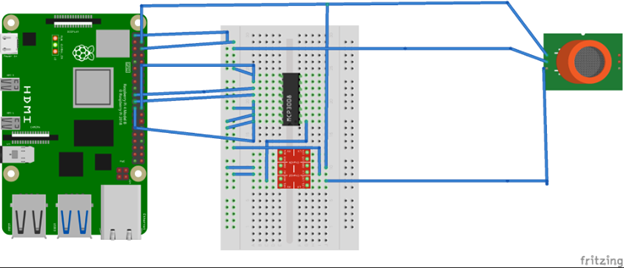
\includegraphics[width=3in]{../assets/schematics/MQ2SensorBB.png}
    \caption{Bread board configuration of the smoke sensor.}
\end{figure}

\begin{figure}[H]
    \centering
    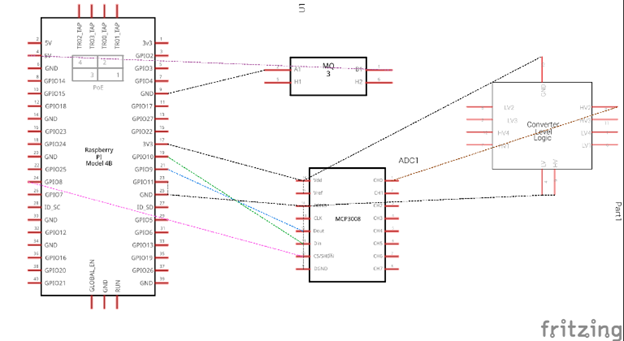
\includegraphics[width=3in]{../assets/schematics/MQ2SensorSchematic.png}
    \caption{Schematic of the smoke sensor circuit.}
\end{figure}

\subsection{LCD Display}

The project incorporates a 16x2 character LCD Display for real-time monitoring, utilizing the I2C communication
protocol for easy interfacing with the Raspberry Pi . This display operates on either 5V or 3.3V and is used to flash
in an emergency to indicate as smoke levels and temperature rise directly to the user. The choice of an LCD display
ensures that information about the environmental condition is immediately accessible, providing a quick overview
without needing to access the system digitally.

\begin{figure}[H]
    \centering
    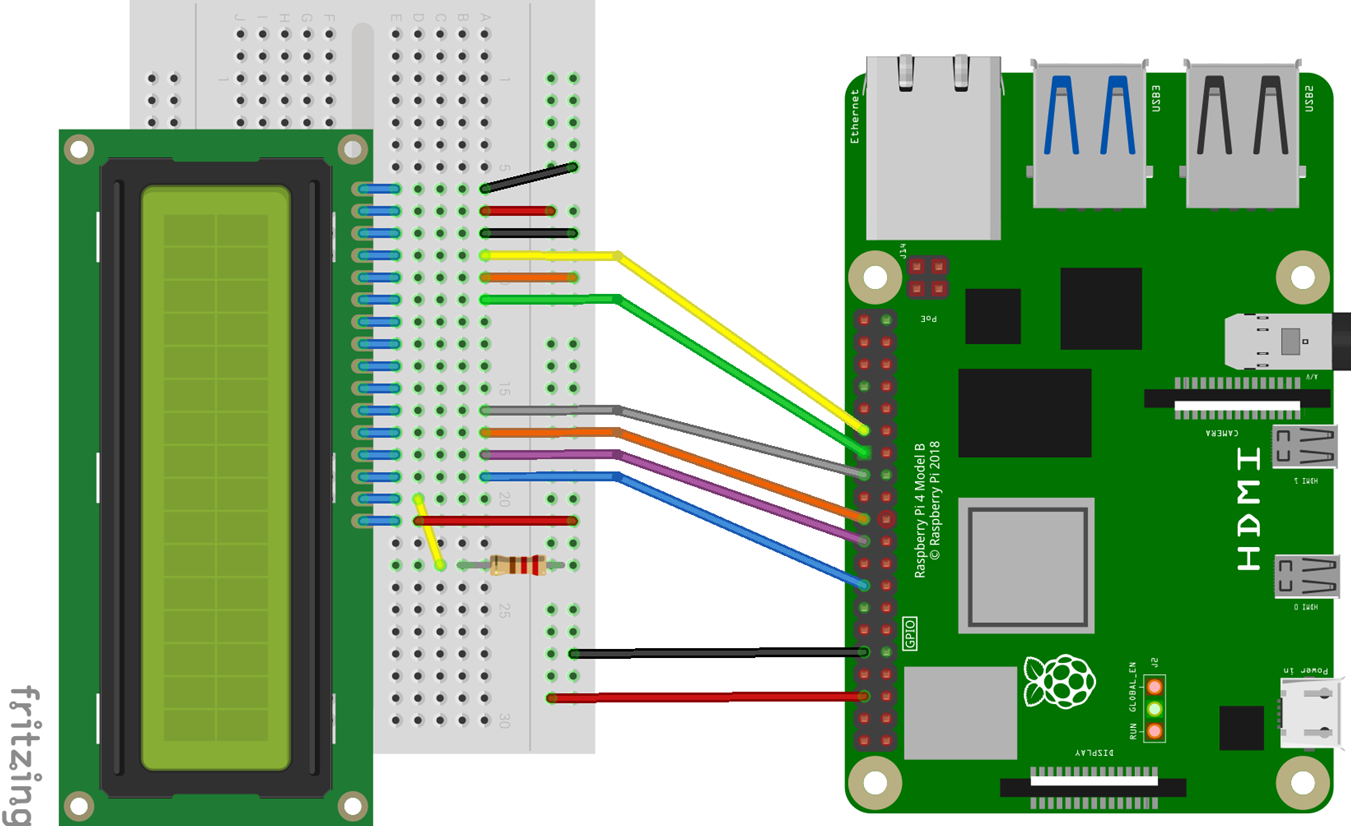
\includegraphics[width=3in]{../assets/schematics/LCDBB.png}
    \caption{Bread board configuration of the LCD display.}
\end{figure}

\begin{figure}[H]
    \centering
    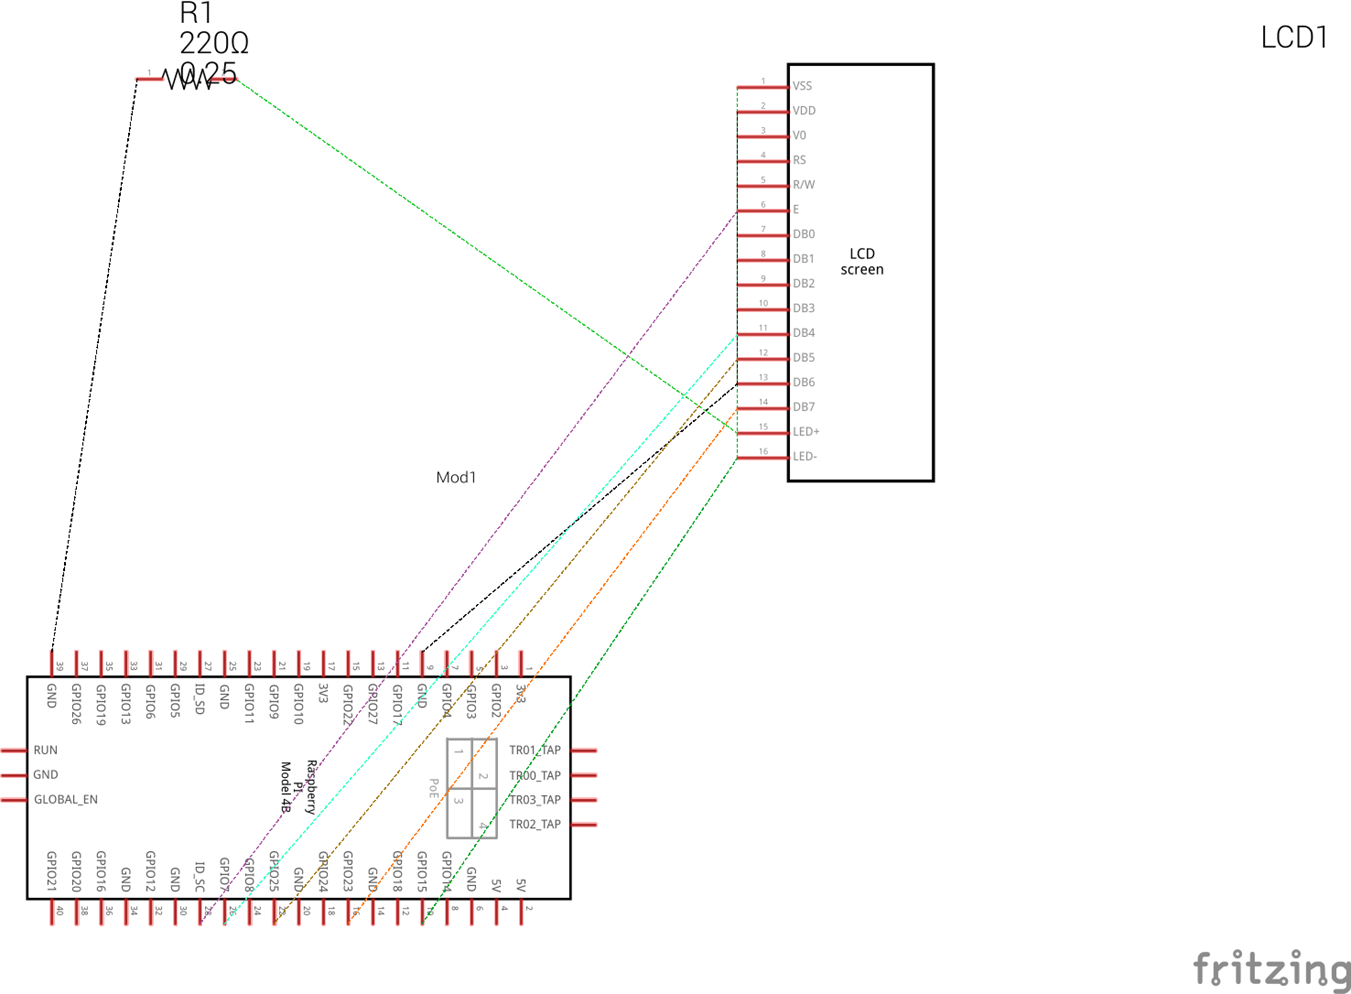
\includegraphics[width=3in]{../assets/schematics/LCDSchema.png}
    \caption{Schematic of the LCD display circuit.}
\end{figure}

\subsection{Piezoelectric Buzzer}

The inclusion of a simple piezoelectric buzzer in the system design offers an effective way to generate audible alerts
when smoke or high temperatures are detected. Operating between 3.3V to 5V and controlled via a GPIO pin, the buzzer
can produce a range of tones, making it a versatile component for different alert types. It ensures that the system can
attract attention through sound, complementing visual alerts and enhancing the overall effectiveness of the fire
detection system.

\begin{figure}[H]
    \centering
    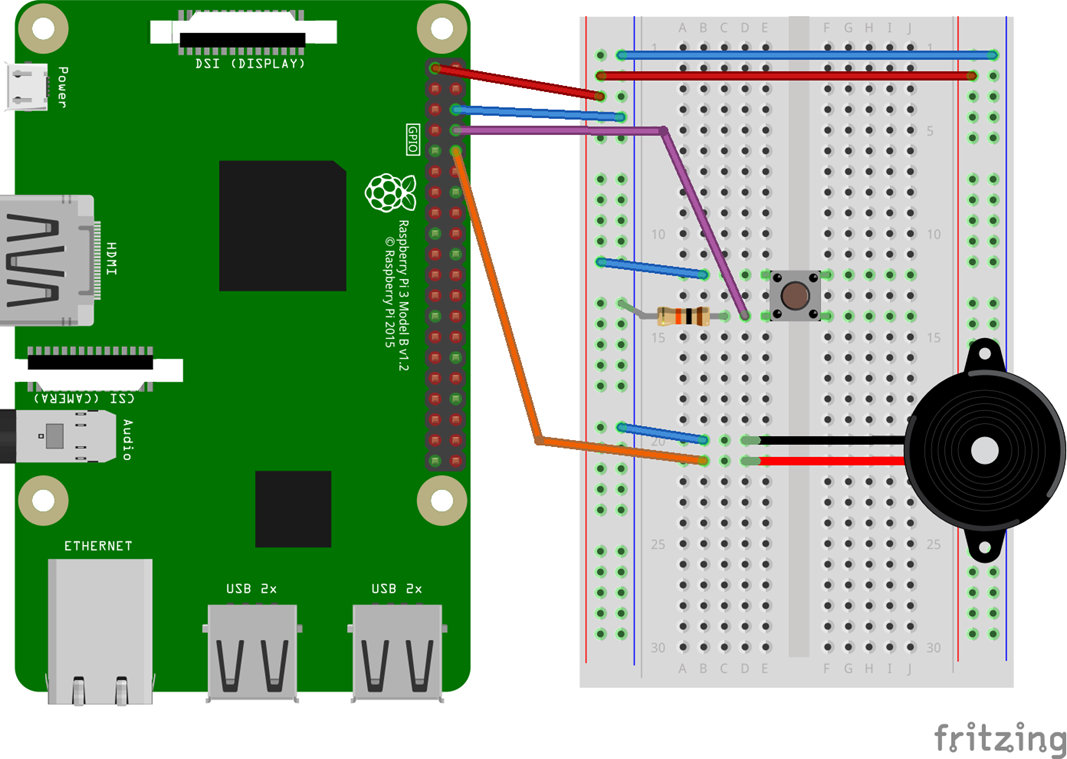
\includegraphics[width=3in]{../assets/schematics/BuzzerBB.png}
    \caption{Bread board configuration of the piezoelectric buzzer.}
\end{figure}

\begin{figure}[H]
    \centering
    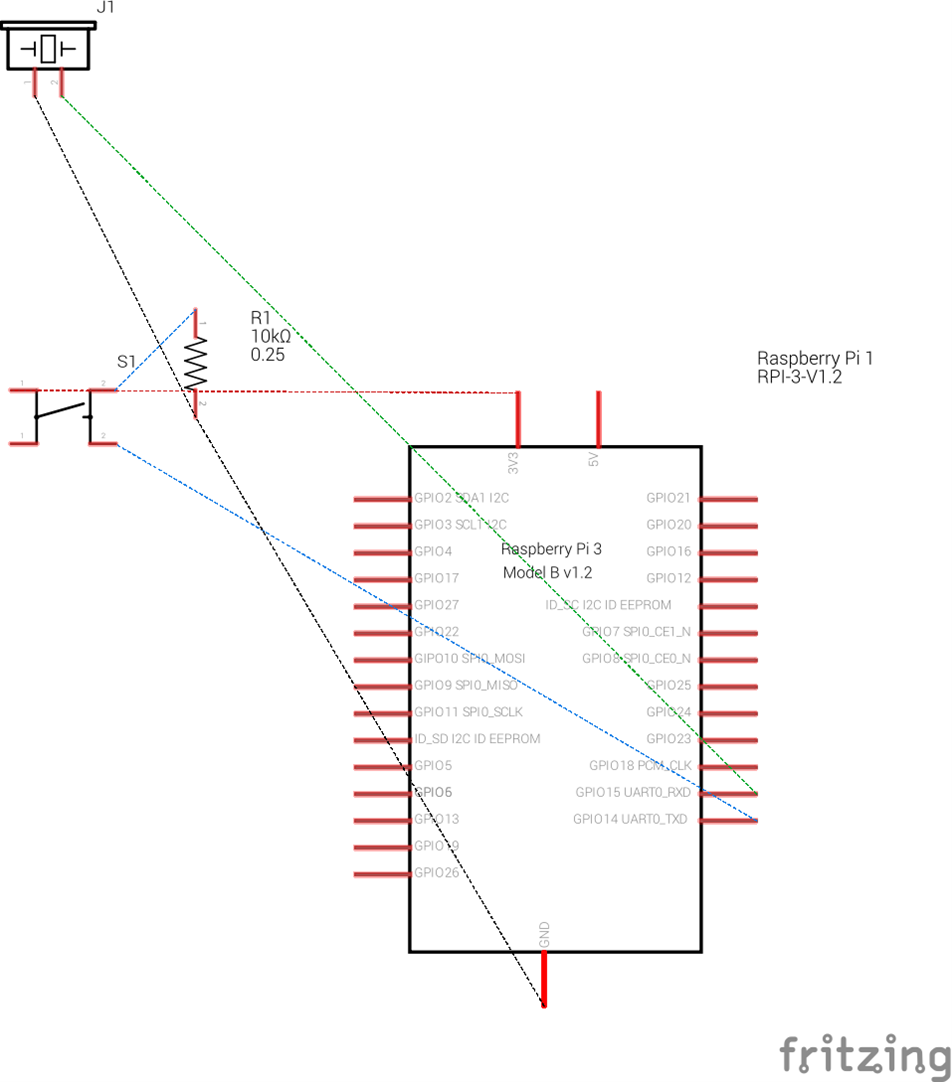
\includegraphics[width=3in]{../assets/schematics/BuzzerSchema.png}
    \caption{Schematic of the piezoelectric buzzer circuit.}
\end{figure}

The following schematics show the connections between the piezoelectric buzzer and the Raspberry Pi Pico. There is no
Fritzing footprint for the Pi Pico, so the Raspberry Pi 4 is used as a placeholder.

\begin{figure}[H]
    \centering
    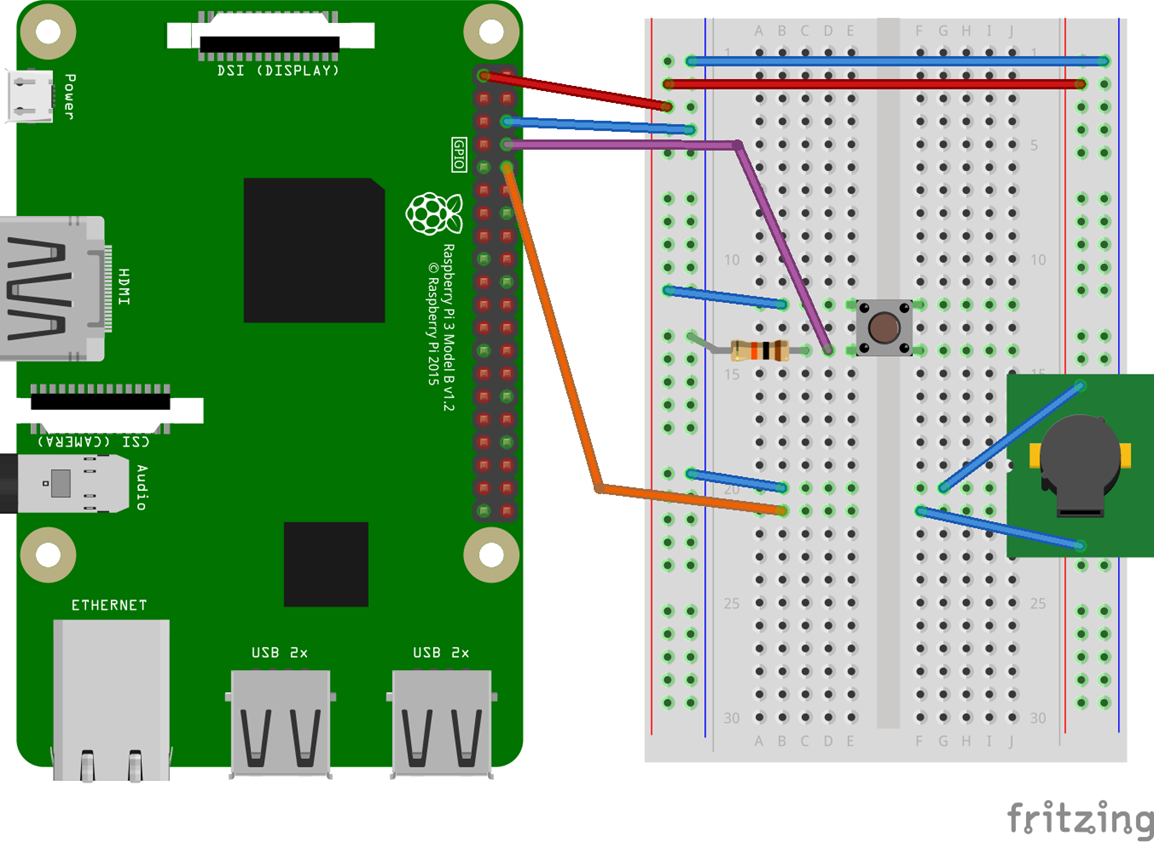
\includegraphics[width=3in]{../assets/schematics/AudiohatBB.png}
    \caption{Bread board configuration of the piezoelectric buzzer with the Pi Pico.}
\end{figure}

\begin{figure}[H]
    \centering
    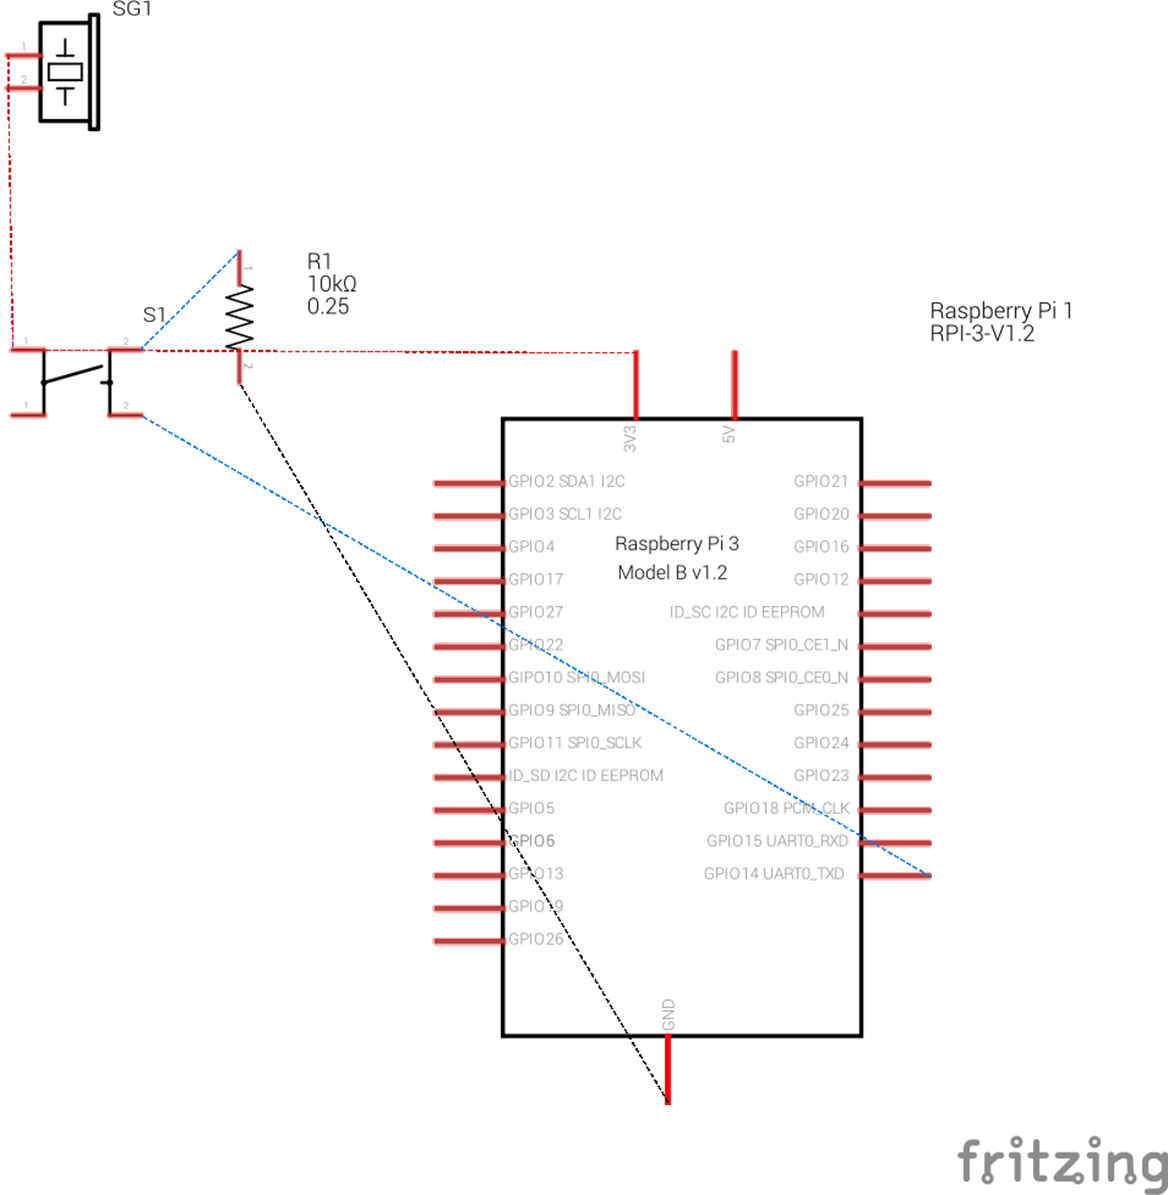
\includegraphics[width=3in]{../assets/schematics/AudiohatSchema.png}
    \caption{Schematic of the piezoelectric buzzer circuit connected to the Pi Pico.}
\end{figure}

\section{GUI Design}

\subsection{Table of Users/Roles}

\section{Test Plans}

Testing is an important part of any system's design. It ensures that project iterations follow the specification,
behave appropriately and are less likely to include bugs.

\subsection{End-to-end Communication Demo}

The end-to-end communication demo should demonstrate all of the major forms of communication present in the FANS
system. In order to achieve this level of demonstration, the following communication examples will be showcased:

\begin{itemize}
    \item Sensor data upload to Firebase over internet.
    \item Email notifications to affected users over internet (email protocol).
    \item Haptic alarm buzzing in accordance with emergency flag in Firebase over internet.
    \item Display of sensor data on the user interface over internet.
    \item Emergency signal from sensor data collection system to the alarm system on local network.
\end{itemize}

It should be noted that the test for the sensor data upload over internet also demonstrates I2C communication between
the Pi 4 and the SenseHat board.

First is the uploading of sensor data to the Firebase database over the internet. For this communication sequence, the
sensor data collection system will be run on one of the Raspberry Pis. It will read temperature data from the SenseHat
and post this data to the Firebase database using Pyrebase. The demonstration can be verified by watching the Firebase
database console, since the data will be updated in real-time.

Second will be the email notifications to affected users over the internet using email protocol. To achieve this
demonstration, the email notification system will be run on one of the Raspberry Pis. Using Pytest, the program will
first send an email from the FANS email back to itself. Then, the program will use \texttt{imaplib} to login to the
FANS email account and verify that the latest message in its inbox contains the same email message that was sent in the
test. If the messages match, Pytest will report a success. This test is fully automated.

Next is the haptic alarm buzzing. For this test, the haptic alarm program will be run on one of the Raspberry Pi's to
emulate the Pi Pico (as it has not arrived at the time of writing). When the program is run, it will poll the Firebase
database using \texttt{pyrebase} to check if the emergency flag has been raised. The flag can either be raised by hand
(the tester modifies the flag using the Firebase console) or it can be set by running the sensor data collection system
with a low emergency reporting threshold for temperature. In either case, when the flag is raised, the output of the
haptic alarm can be verified by observing the console messages. Console printing will be used in place of the buzzer
actuator while we wait for components. A console message of "buzz" would indicate the buzzer buzzing, and no console
messages indicate no emergency while the alarm is polling the database.

To test the display of sensor data collection on the user interface, the GUI will be run on one of the Raspberry Pis
using Flask. When a user clicks the "refresh" button, the Flask API endpoint responsible for returning temperature data
will be hit. The endpoint will use \texttt{pyrebase} to request the latest temperature data from Firebase and then will
respond with JSON. The GUI's JavaScript logic will simply print this JSON as text content of an HTML paragraph tag to
show that the connection is present.

Finally, to demonstrate UDP communication over the local area network, both the sensor data collection system and the
alarm system will be run on two separate Pis. Both programs will first upload their public IP to the Firebase database
under a 'devices' table, and then read the other device's IP. The sensor data collection system should have a
sufficiently low emergency threshold to trigger an emergency at room temperature (only for testing purposes). Once the
sensor data collection system detects an emergency, it will send a UDP message containing the numerical data '0' (the
agreed upon encoding for signifying an emergency) over the LAN addressed to the alarm system. The alarm system will
receive the emergency notification, and instead of activating an actuator it will print "Received 0" to the console.
This can be manually verified.

\subsection{Unit Test Demo}

The purpose of the unit test demo is to demonstrate that the individual components of our system behave as expected and
do not contain logical or physical errors. This will sanity check our hardware components and our software logic.

\subsubsection{Hardware}

The hardware components that will need to be tested are:

\begin{itemize}
    \item Smoke sensor
    \item Temperature sensor
    \item Piezoelectric buzzer
    \item LCD screen
\end{itemize}

\textbf{Smoke Detector}

The smoke detector will be difficult to test due to the nature of what it measures. It will not be possible to light a
fire within the school or near campus because that will set of existing fire suppression systems and may be dangerous.
Testing the smoke detector in smokey environments can be done by:

\begin{itemize}
    \item Running the data collection from the smoke detector in a smoking zone on campus.
    \item Running the data collection from the smoke detector off campus and lighting a fire nearby.
\end{itemize}

For both of these tests, it should be verified that smoke levels are detected. This will be a one-time sanity test of
the sensor. The smoke detector can also be tested in smokeless environments by collecting data from the sensor indoors
on campus and ensuring that no smoke is detected.

\textbf{Temperature Sensor}

To test the temperature sensor, we can collect data from the sensor in the lab setting and ensure that measurements are
within the acceptable range for room temperature.

\textbf{Piezoelectric Buzzer}

To test the piezoelectric buzzer, we can test turning on and off the buzzer and verifying that it produces noise.
Additionally, we can set the buzzer to produce different frequencies and verify that they are set correctly by checking
with a instrument tuning app.

\textbf{LCD Screen}

Finally, to test the LCD screen, several test messages can be displayed on screen and visually inspected for
correctness as a sanity check.

\subsubsection{Database Integrity}

To test cloud database integrity, we can perform several test and security checks.

\textbf{Insecure Access}

To test the security of the cloud database, we can attempt to perform read and write operations using an incorrect API
key and ensure that the requests are denied.

\textbf{Stress Test}

To stress test the cloud database, several instances of the sensor data collection program can be run on multiple
Raspberry Pis, all of which will upload sensor data to the database. The database should:

\begin{itemize}
    \item Keep up with all of the simultaneous requests.
    \item Avoid any overwriting/race conditions with concurrent write operations.
\end{itemize}

\subsubsection{Software}

% TODO: Write unit test plans for the software

\subsection{Final Demo}

% TODO: Write final demo

\section{Project Update}

\subsection{Project Milestones}

\subsection{Schedule of Activities}


% BIBLIOGRAPHY %
\pagebreak
\printbibliography

\end{document}
